\section{Wrapfigure}

\begin{wrapfigure}{r}{0.2\textwidth}
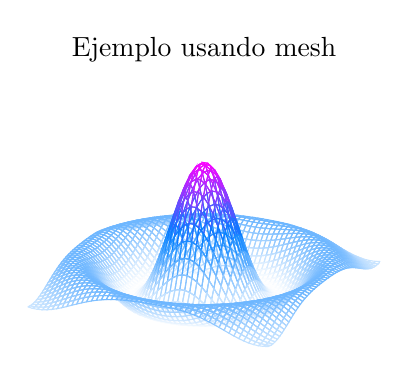
\begin{tikzpicture}
            \begin{axis}
                [
                title=Ejemplo usando mesh,
                hide axis,
                colormap/cool, 
                width=0.5\textwidth]
            \addplot3[mesh,samples=50,domain=-8:8,]{sin(deg(sqrt(x^2+y^2)))/sqrt(x^2+y^2)} ;
            %\addlegendentry{\(\frac{sin(r)}{r}\)}
            \end{axis}
        \end{tikzpicture}
\end{wrapfigure}        
\lipsum[1-4]
\begin{wrapfigure}{l}{0.5\textwidth}
\begin{tikzpicture}
\begin{axis}
[
    title={Contour plot, view from top},
    view={0}{90}, width=0.5\textwidth
]
\addplot3[
    contour gnuplot={levels={0.8, 0.4, 0.2, -0.2}}
]
{sin(deg(sqrt(x^2+y^2)))/sqrt(x^2+y^2)};
\end{axis}
\end{tikzpicture}
\end{wrapfigure}
\lipsum[1-4]

\section{Figuras en 3D intersecadas}

\begin{figure}
    \centering
    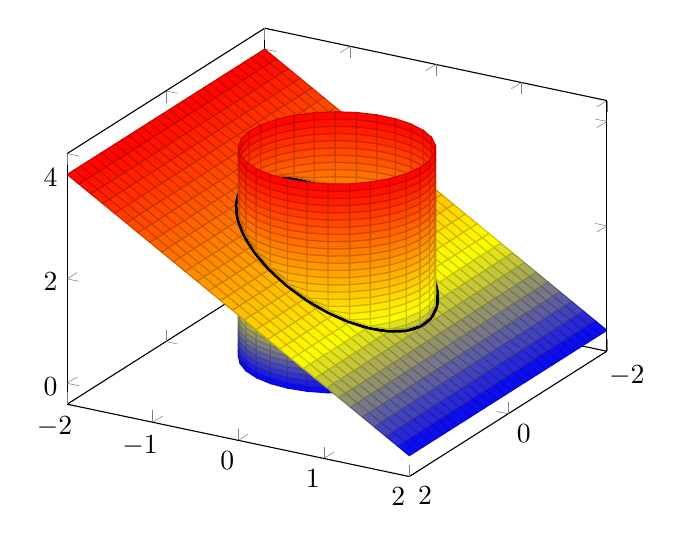
\begin{tikzpicture}
        \begin{axis}
            [view={120}{30}]
            % parte baja del cilindro
            \addplot3[surf,z buffer=sort,samples=30,variable=\u,variable y=\v,domain=0:360,y domain=0:3]
            ({cos(u)},{sin(u)},{min(2-y,v)});
            %plano
            \addplot3[surf, z buffer= sort,samples=30,variable=\u,variable y=\v,domain=-2:2,y domain=-2:2]({u},{v},{2-v});
            %interseccion
            \addplot3[color=black,smooth,samples=30,variable=\u,domain=0:360,line width=2.5pt]
            ({cos(u)},{sin(u)},{2-sin(u)});

            %parte alta cilindro
            \addplot3[ surf,z buffer=sort,samples=30,variable=\u,variable y=\v,domain=0:360,y domain=0:4]
            ({cos(u)},{sin(u)},{max(2-y,v)});
    
        \end{axis}
    \end{tikzpicture}
    \caption{Caption}
    \label{fig:enter-label}
\end{figure}